\section{Text Analysis}
\subsection{Text Data Access}
L'obiettivo principale del text data access è di connettere user con le giuste informazioni al momento giusto. Questa operazione può essere svolta in due modi: \begin{itemize}
    \item pull, dove l'user prende l'iniziativa di cercare le info ed estrapolarle dal sistema
    \item push, dove il sistema prende l'iniziativa e offre informazioni all'user. 
\end{itemize}
Ci sono due modi per interrogare una collezione di dati, il \textit{search engine} e \textit{sistema di raccomandazione}. Nel primo caso siamo noi a dare la query. Nell'altro caso, è tipo su netflix che consiglia delle serie. Quindi pull è il search engine, push è raccomandazione. Prende il nome di \textit{Text retrieval} quello che noi abbiamo appena descritto come search engine, ovvero trovare un informazione tramite query. 
\\
Problema solitamente complesso: non è una semplice query in un database che fornisce un risultato esatto. La risposta desiderata è anche soggettiva, dipende dalla correttezza della query scritta dall'utente (basta pensare alla ricerca su Google e come cambiano i risultati sulla base di ciò che si cerca). 

\subsection{Text Retrieval}
Data una collezione di documenti, il text retrieval può essere definito come: utilizzando una query dell'user, (per esempio, una \textit{descrizione} dell'informazione ricercata) identificare un subset di documenti che soddisfano la richiesta. 
\begin{itemize}
    \item Abbiamo V vocabolario di tutte le parole di un natural language.
    \item q, query dell'user, dove $q_i$ $\in$ V
    \item $d_i$, documento tale che $d_{ij}$ $\in$ V
    \item la query è più corta del documento
    \item una collezione C è l'insieme di documenti d
    \item assumiamo che esista un sottoinsieme R di documenti, che sono rilevanti per la query q
\end{itemize}
Il sottoinsieme perfetto R(q) non è sempre il risultato. Per correttezza, considereremo un R'(q), come un'approssimazione del risultato esatto R(q) comunque accettabile. 
\\
\textbf{Come possiamo trovare quindi R'(q)?} Esistono due metodi: \textit{document selection} o \textit{document ranking}.

\subsubsection{Document Selection vs Document Ranking}
La document selection utilizza un classificatore binario per classificare se un documento è relevant o no rispettando una particolare query. Usando questa strategia, il sistema capisce l'effettiva rilevanza di un documento. 
\\
Nel document ranking, abbiamo una funzione di ranking e l'user sceglie un limite. In questo caso, il sistema impara una rilevanza relativa: quali documenti potrebbero essere rilevanti. Per il principio del probability ranking, fare un ranking decrescente di rilevanza fornisce una informazione utile se l'utilità di un documento per l'user è indipendente dall'utilità degli altri documenti e se l'user potrà guardare la lista dei risultati sequenzialmente.

\subsection{Retrieval Models}
Esistono diversi modelli per fare retrieval, e si distinguono per tipologia di approccio al problema. Alcuni sono basati sempre sul concetto di similarità, altri lavorano sul piano probabilistico. Molti modelli si basano anche sulla consapevolezza che i documenti di testo vengono rappresentati come bag of words, non shingles. Si sceglie un vocabolario (lingua) di riferimento e si usa quello.
\\
\begin{figure}[th]
    \centering
    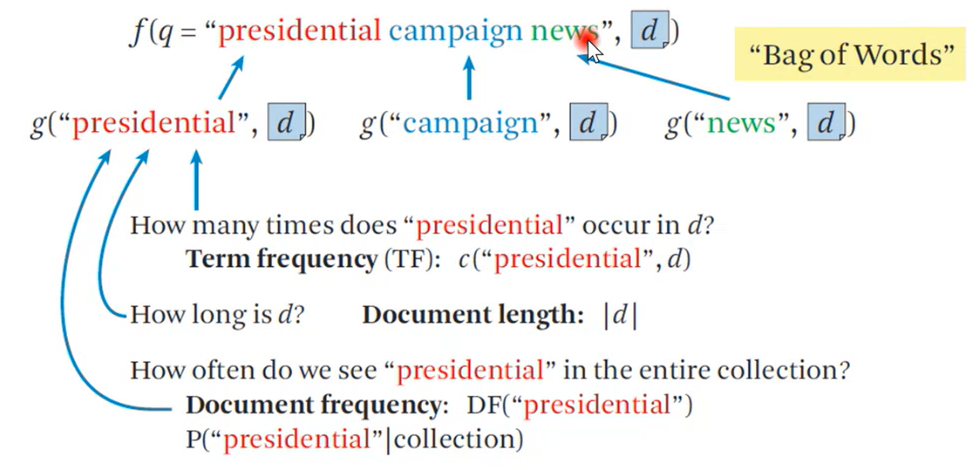
\includegraphics[scale=0.5]{Text Analysis/img/bagofwords.png}
\end{figure}
\\
Ma allora come faccio a decidere quale documento è più importante? Per esempio posso contare le occorrenze della parola ricercata, oppure tenere conto quanto è lungo il documento, poichè più parole ci sono, più è probabile che almeno una delle parole della mia query compaia nella ricerca; un ultimo valore che è necessario conoscere sono le stop words: parole "inutili". Quando, quanto ecc... sono parole che non ci interessano quindi le eliminiamo. Poi ci sono parole importanti, che dipendono dal dominio della ricerca. In un documento di calcio, "Goal" è una parola molto frequente, meno discriminatoria nella ricerca. Ma una parola come "Messi", è molto più specifica. Questo effetto prende il nome di document frequency (spiegato meglio in seguito). 
\\
Le metriche più importanti sono sicuramente \textbf{term frequency} e \textbf{document frequency} quando si parla della funzione di ranking (che chiameremo TF e DF).

\subsubsection{Vector Space Retrieval Model}
Modello molto semplice basato sulla similarità che trasforma i documenti della collezione in vettori e anche la query dell'utente. 
\\
\begin{figure}[th]
    \centering
    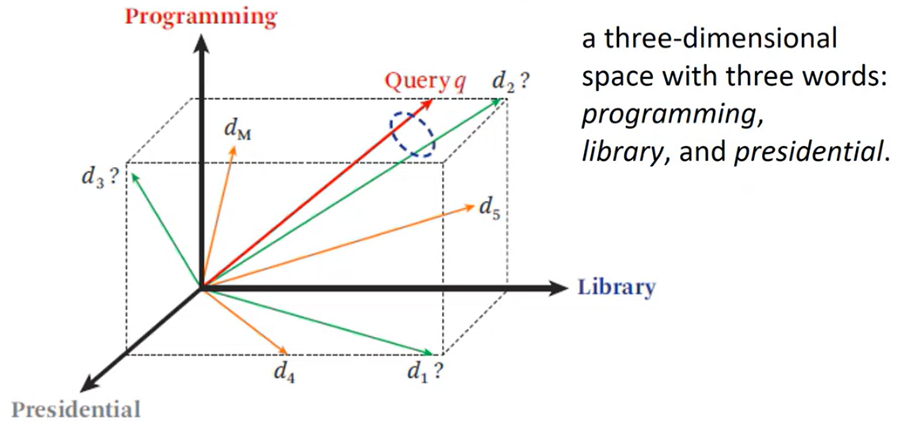
\includegraphics[scale=0.5]{Text Analysis/img/vector space retrieval.png}
\end{figure}
\\
Vado ad orientarli nello spazio e guardo quelli che sono più vicini al vettore della query. Per esempio nell'immagine parliamo di d2. 
\\
\textbf{Come trasformiamo una query in un vettore?} Stabilisco un vocabolario, di parole, ogni parola è una componente e ha una misura che dipende dalle occorrenze della parola. Dopo è necessario calcolare la distanza: coseno dell'angolo sotteso tra i due vettori. Più i vettori sono allineati, più l'angolo tende a 0, più il coseno tende a 1, \textit{più i vettori sono simili}. 
\\
Vediamo ora le tecniche per la ricerca di similarità utilizzando questo modello:
\begin{itemize}
    \item Vector Space Model Booleano: mi rappresenta le parole con 1 se è presente, 0 se non è presente. Utilizziamo poi il dot product per trovare la similarità: Sim(q,d) = q.d = $\sum_{i=1}^{N} x_i y_i$ dove le x sono in q, e le y sono in d. Non funziona quasi mai purtroppo, perchè è troppo semplice non considera il TF.
    \item Improved VSM Instantiation: miglioriamo la tecnica precedente aggiungendo TF. Non consideriamo più l'i-esimo elemento di q e d come 1 o 0 in base alla presenza della parola ma lo sostituiamo con il numero di volte che essa compare.  
    \item IDF Approach: non basta nemmeno aggiungere TF, allora mettiamo anche IDF che è l'inverso della DF. Utilizziamo la IDF perchè la DF sarebbe il numero di elementi in cui una certa parola appare, ma vogliamo penalizzare le parole che appaiono in troppi documenti, quindi usiamo il suo inverso. 
    \begin{center}
        \begin{math}
            IDF(w) = \frac{M+1}{DF(w)}
        \end{math}
    \end{center}
    E usiamo il suo logaritmo per smorzare alcuni valori troppo elevati. Ottenuto tale valore comunque, sfruttiamo TF come prima ma ci moltiplichiamo IDF che funge da peso. 
    \begin{center}
        \begin{math}
            f(q,d) = \sum_{i=1}^{N} x_i y_i = \sum c(w, q) c(w, d) log(\frac{M+1}{DF(w)})
        \end{math}
    \end{center}
    \item TF Transformation: l'approccio descritto nel punto precedente ha comunque un problema, la probabilità varia linearmente all'aumentare di TF; per esempio basta che la parola "cipolla" sia presente 2 volte che quel documento ottiene una probabilità doppia rispetto ad un documento dove appare una sola volta. Per compensare andiamo a smorzare TF ad esempio mettendo 1+log(1+TF).
    \item State-of-Art VSM Ranking Functions: pivoted lenght e BM25 si basano su altri parametri aggiunti che modificano il TF. BM25 sfrutta questa formula: 
    \begin{center}
        \begin{math}
            y = \frac{(k+1)TF}{TF+k}
        \end{math}
    \end{center}
    Dove k+1 è il valore massimo che il TF può raggiungere. Se non è presente la parola, vale 0, altrimenti tenderà a k+1. Pivoted lenght si basa invece sulla lunghezza del documento. 
\end{itemize}

\newpage    

\subsection{Probabilistic Retrieval Models}
Determinare, dato il documento e data la query, quanto esso sia rilevante. Si vede bene in questo esempio:
\\
\begin{figure}[th]
    \centering
    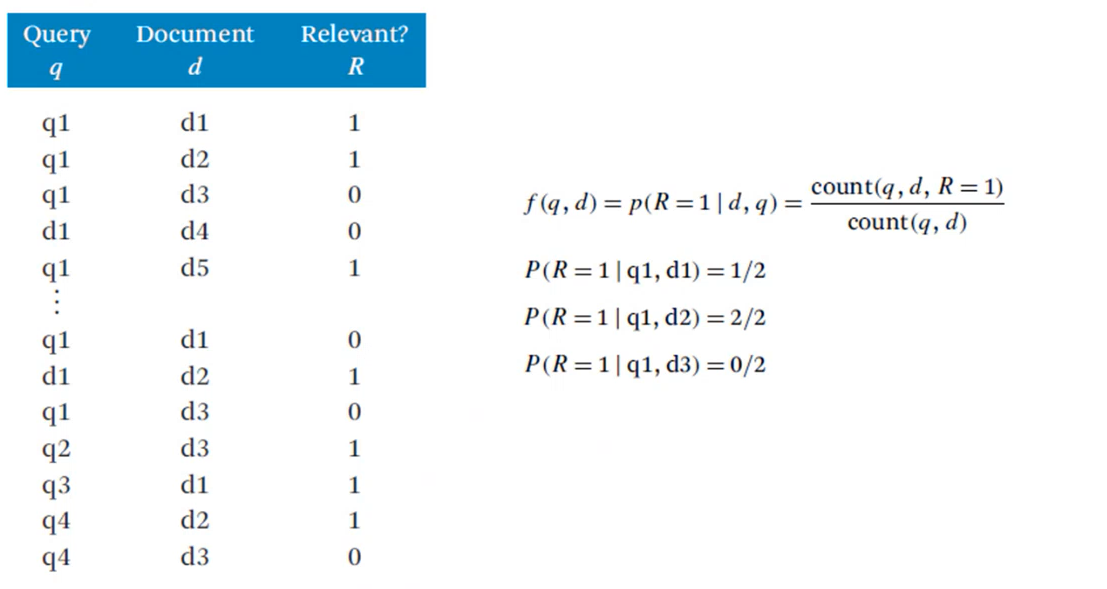
\includegraphics[scale=0.5]{Text Analysis/img/example.png}
\end{figure}
\\
Confronta più risposte sulla domanda di rilevanza, come se confrontassi la risposta di più utenti. Approssimiamo la rilevanza alla probabilità:
\begin{center}
    \begin{math}
        p(R=1|d,q) = p(q|d,R=1)
    \end{math}
\end{center}
Della query, data una rilevanza e un documento. Quindi la domanda diventa:
\begin{center}
    \textit{Qual è la query che mi dà come risultato tale documento?}
\end{center}
Perchè è vantaggioso? Posso stimare le query ipotetiche, senza averne necessariamente una. 

\subsubsection{Text statistics: Zipf's Law}
Il rank di una parola moltiplicato per la frequenza di tale parola è una costante.
\begin{center}
    \begin{math}
        r \times f = k
    \end{math}
\end{center}
Quello che dice questa legge, nello specifico, è che ci saranno poche parole che appaiono tantissimo (le parole più frequenti) ma si decresce in maniera non lineare, quindi ci saranno tantissime parole che appaiono pochissimo. 

\subsubsection{Language Model}
Il language model è una probabilità che io assegno ad una frase. Si suddivide in:
\begin{itemize}
    \item machine translation: traduzione linguistica corretta
    \item correzione di pronuncia 
    \item speech recognition: p(I saw a van) $>>$ p(eyes awe of an)
\end{itemize}
E tanti altri. Nel probabilistic language modeling l'obiettivo è quello di calcolare la probabilità di una frase o sequenza di parole. In questo modo, un'altra task correlata è sicuramente la prediction della upcoming word. 
\\
A livello matematico, l'obiettivo è quello di calcolare la probabilità di una parola w data una history h = $p(w|h)$; per farlo ci possiamo affidare alla \textit{chain rule of probability}, cerchiamo di suddividere il problema, dove la probabilità di una frase diventa:
\begin{center}
    \begin{math}
        P(A,B,C,D) = P(A)P(B|A)P(C|A,B)P(D|A,B,C)
    \end{math}
\end{center}
Ma non arriviamo ad un grande risultato perchè con frasi troppo lunghe sono troppo complesse. Dobbiamo usare dei bigrammi! Usiamo solo l'elemento precedente. Quindi in un documento invece di andare a visualizzare intere frasi, guardiamo solo la parola che precede. Il calcolo della probabilità, in quel caso, diventa: 
\begin{center}
    \begin{math}
        P(w_i | w_{i-1}) = \frac{count(w_{i-1}w_i)}{\sum count(w_{i-1}w)}
    \end{math}
\end{center}
Ovvero la probabilità della coppia che sto esaminando, diviso il numero di correlazioni tra la parola precedente e un'altra qualsiasi parola che non sia quella giusta. Il discorso è comunque analogo nel caso di trigrammi, o nel caso considerassimo k parole alla volta con k $>$ 3. 
\\
\textbf{Come è cambiata con il machine learning?} Non è capace, un modello machine learning non riesce con troppi dati, ma una rete neurale sì. 
\\
Ovviamente vado poi a moltiplicare (come mostrato in alto) la probabilità di ogni bigramma fino ad ottenere la probabilità di una frase. 
\\
\begin{figure}[th]
    \centering
    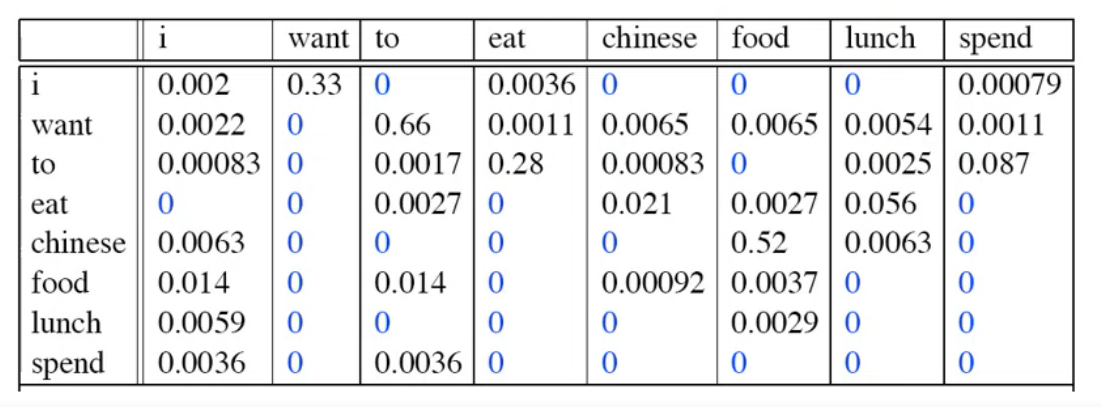
\includegraphics[scale=0.45]{Text Analysis/img/bigrams.png}
\end{figure}
\\
In questa immagine è possibile visualizzare un esempio di calcolo su bigrammi. Una domanda sorge spontanea, come vengono gestiti gli 0? Potrebbero dare problemi di generalizzazione! Allora per evitare che ci sia uno 0, possiamo utilizzare la tecnica di Laplace Smoothing, per cui aggiungiamo un 1 al conteggio di tutto. 
\\
\begin{figure}[th]
    \centering
    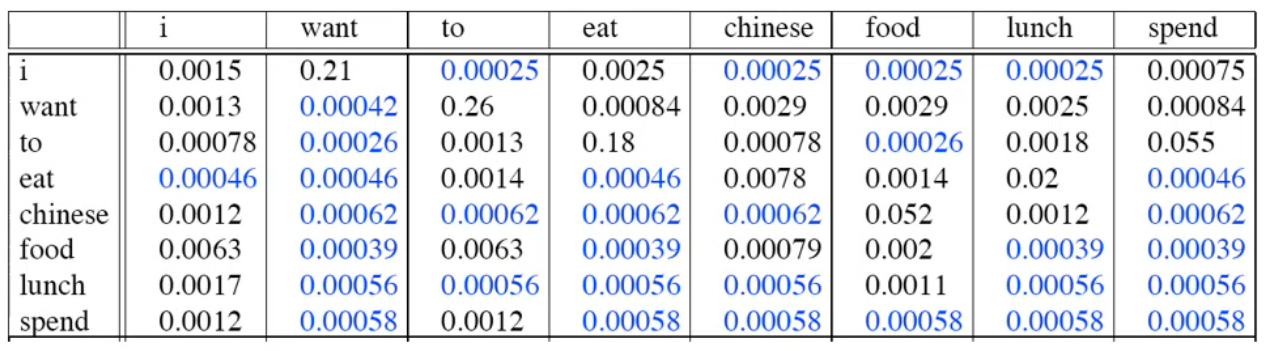
\includegraphics[scale=0.45]{Text Analysis/img/laplacesmoothing.png}
\end{figure}
\\
I risultati della tabella cambiano di tanto! E non solo gli zeri.

\newpage

Quello che avviene infatti nel Laplace Smoothing non è solo un aumento di 1 del conteggio, ma quando vado a calcolare le probabilità:
\begin{center}
    \begin{math}
        P(w_i | w_{i-1}) = \frac{count(w_{i-1}w_i) + 1}{\sum count(w_{i-1}w) + V}
    \end{math}
\end{center}
Al denominatore vado anche a mettere il vocabolario V. Quindi il conteggio nelle tabelle, prima e dopo Laplace, cambia: 
\\
\begin{figure}[th]
    \centering
    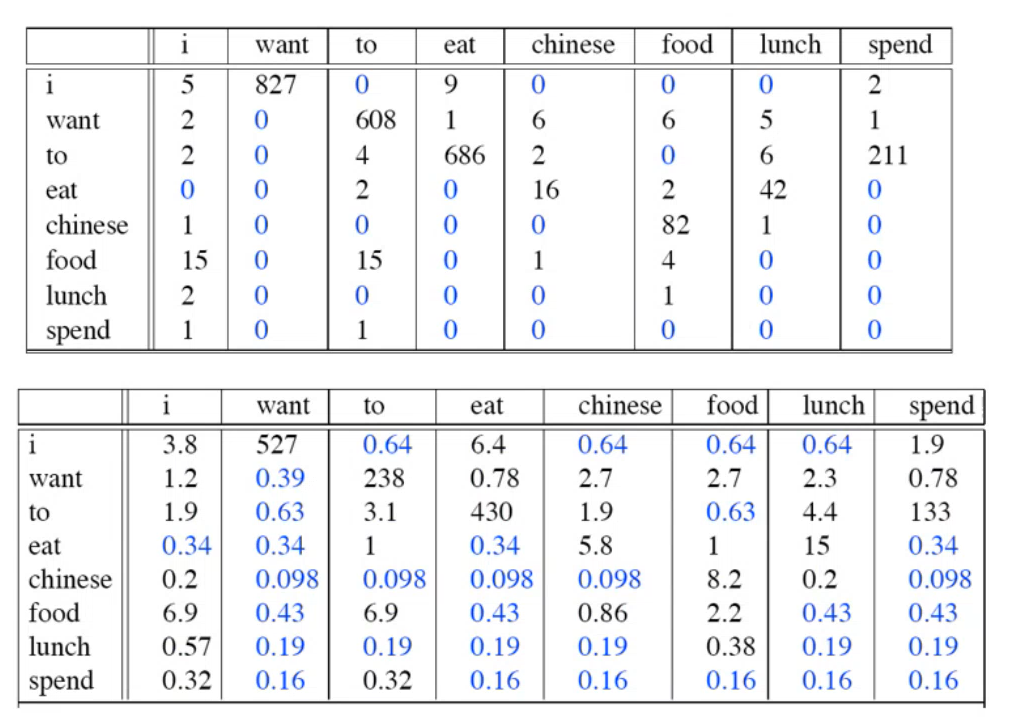
\includegraphics[scale=0.45]{Text Analysis/img/compare.png}
\end{figure}
\\
Ed è dovuto al fattore di discount d:
\begin{center}
    \begin{math}
        d = \frac{c^*}{c} 
    \end{math}
\end{center}
Dove:
\begin{center}
    \begin{math}
        c^* = (ci+1)\frac{N}{N+V} 
    \end{math}
\end{center}

\newpage

